\section{Lessons Learned}\label{sec:lessons_learned}

After over 6 months of weekly meetings, the retrospectives allowed
the process to be improved. Section~\ref{ssub:well} will discuss the
aspects of the \emph{Coding Dojo} that went well. Section~\ref{ssub:less_well}
will discuss the things that worked less well than expected. Finally, in
Section~\ref{ssub:puzzles} the experience of running the sessions in different
contexts and to different audiences raised some issues that are still puzzles
to understand.

\subsection{What Went Well?}\label{ssub:well}

\subsubsection{Retrospectives and Action Items}

As described in the previous section, every meeting ends with a
short retrospective~\cite{Retro}. The participants receive red and yellow sticky
notes and write positive and negative aspects of the session. In the
beginning, the group followed the usual retrospective format,
asking ``What went well?'' and ``What could be improved?''.
These questions led people to write items about the process used for
the meetings, such as when to choose the problem, when to change the
programming language, what laptop to use, etc. This kind of feedback
helped improve the São Paulo \emph{Coding Dojo} itself, reaching the
process described in Section~\ref{subsec:dojosp}.

\begin{figure}[htp]
\centering
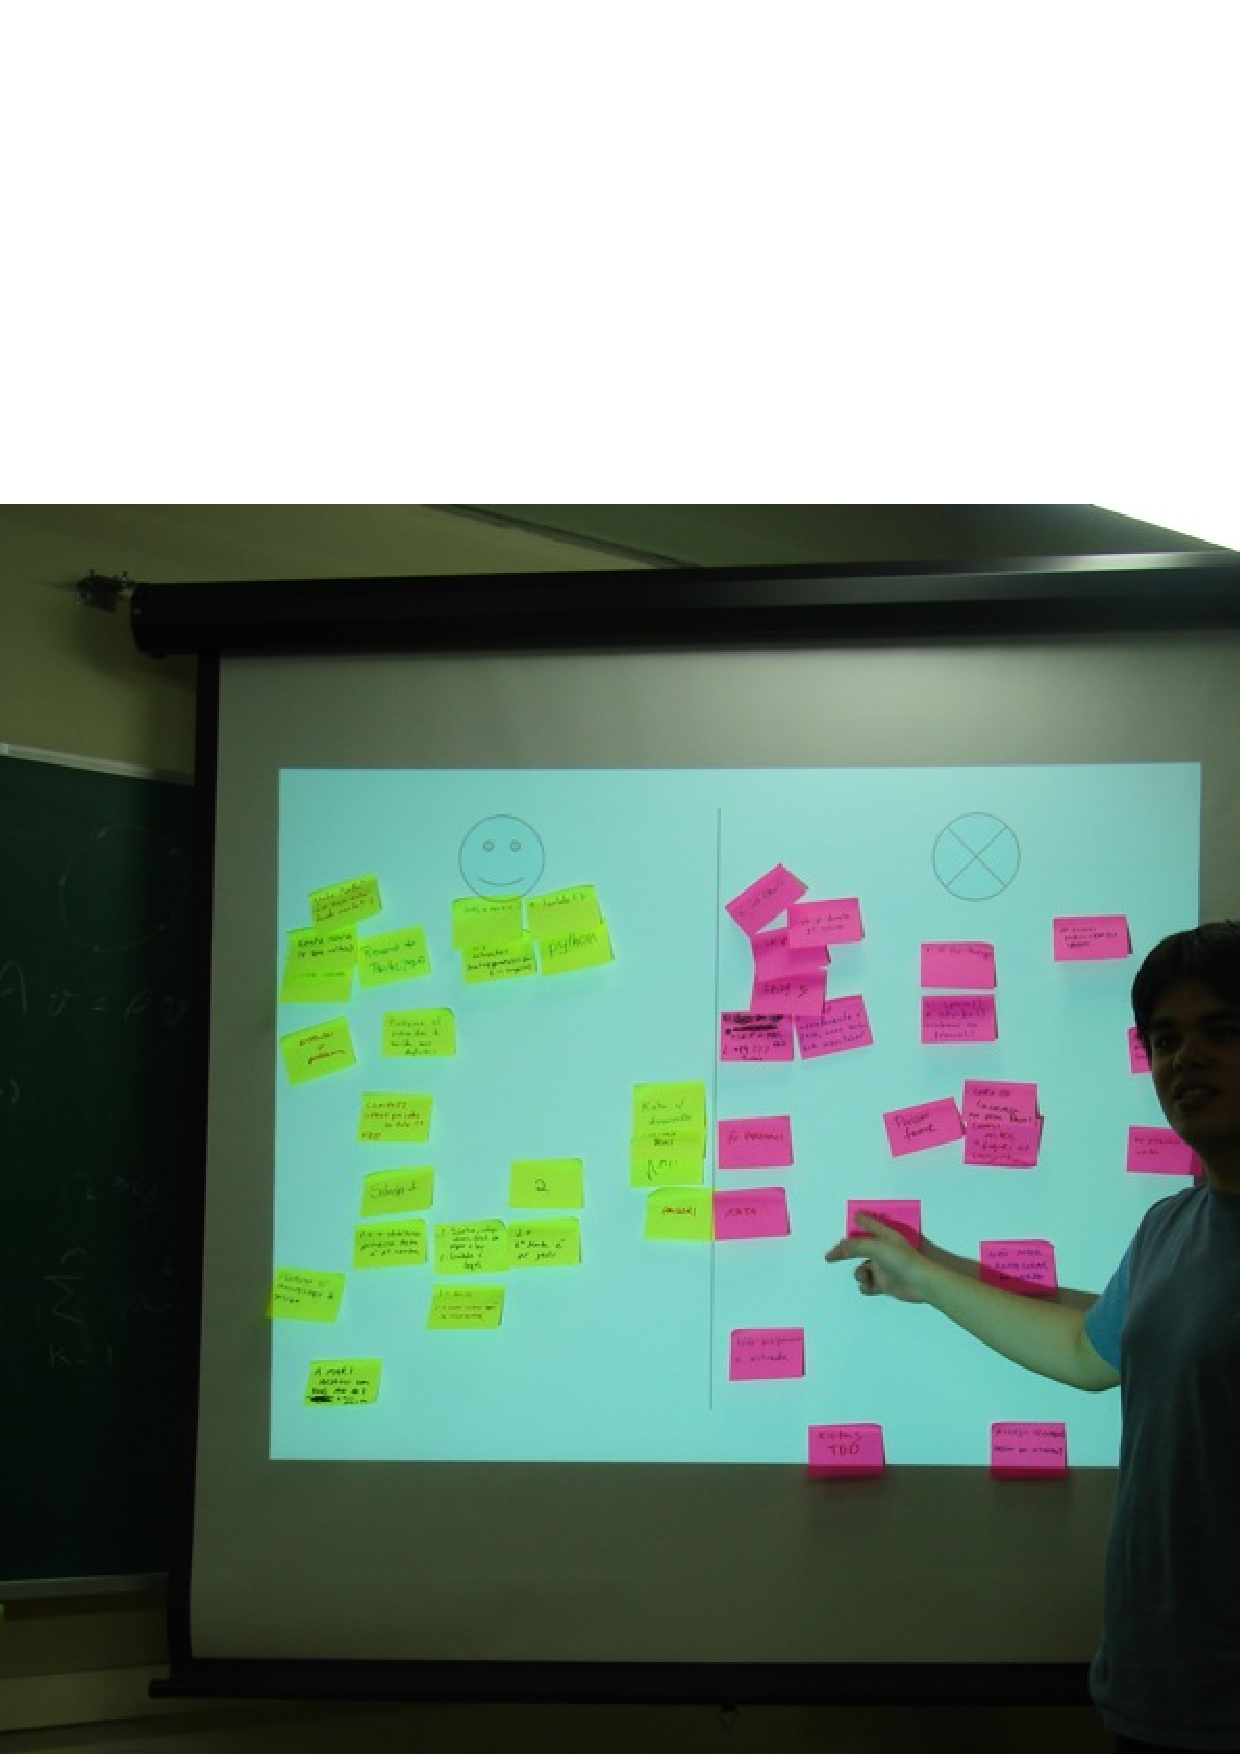
\includegraphics[width=\columnwidth]{retrospective}
\caption{Conducting the retrospective}\label{fig:retrospective}
\end{figure}

After some time, the retrospective format changed to reflect the
objectives of the \emph{Coding Dojo}. Now participants are asked to
think about the following questions:

\begin{itemize}
\item \textbf{``What have we learned?''}: Reflecting and discussing
  what was learned is an effective way to make learning an active
  process and to verify that the session met its goals.
\item \textbf{``What has hindered learning?''}: The negative aspects
  of a meeting are discussed, and the main impediments are
  identified. The group performs a root cause analysis and discusses
	how these impediments could be eliminated, coming up
	with a series of action items. People take responsibility
  to handle each action item for the next meeting, the results are
	recorded for future reflection, and the effects of the change are
	re-evaluated in the next retrospective.
\end{itemize}

\subsubsection{The Goal is not to Finish}

When the São Paulo \emph{Codingo Dojo} started, the participants
agreed that one of the goals was to learn different algorithms and
approaches to problem solving. At the second meeting, during the
\emph{Randori} coding session, the time-boxed rounds became a race
of who could produce more code and get closer to solving the
problem. The coding happened really fast and soon some participants
could not keep up with what changes were made and why.

At the following retrospective, the group decided that finishing the
problem should never be the goal of a meeting. More than that, it was
agreed that not writing the entire solution was OK, as long as the
participants could learn something from the coding session. ``It's OK
not to finish'' has been one of the São Paulo \emph{Coding Dojo}'s
principles ever since, and it is repeated whenever someone joins the
group or simply forgets.

With that principle in mind, the participants take time to write clean and
understandable code, and the group often does not finish implementing the
entire solution to the problems. Unlike a programming challenge or contest,
going fast in a \emph{Coding Dojo} session is not beneficial.

\subsubsection{Time-boxing}

{\Large you say that some ideas have been suggested - I'd like to know
  what these ideas are, and how you plan to try them out.}

The São Paulo \emph{Coding Dojo} has always used 7 minutes time-boxes
for \emph{Randori} sessions. However, for a long time the group
disrespected a bit the time-boxes. That is, if a pair was in the
middle of writing a test or finishing a refactoring, and the group
considered this activity to be short, the pair was allowed to finish
the current code before switching. At first this took 1 or 2 minutes
more, but this overtime gradually increased until there was no more a
time-box, but a minimum time for each pair.

This actually made it difficult for everyone to be focused on the big
picture -- the longer a pair stayed at the front, less and less people
payed attention to them. As a result, the group decided to adopt
\emph{really strict} time-boxes. When the timer rings, no matter
what they are doing, the pair has to be switched. This allowed the
meetings to be more dynamic and easier to follow.

One side-effect of this approach is that if some discussion happens
between the group, the current pair has less coding time. The
participants have not yet found a solution to this, but some ideas
have been suggested and should be attempted at future meetings.

\subsubsection{Information Radiators}

Since the \emph{Coding Dojo} uses TDD, the coding session follows a
clear ``red - green - refactor'' cycle. However, between discussions or
distractions, the group sometimes forgets what is the current
stage. The participants felt the need of visual feedback of the
current stage, such as an information radiator on an XP team. Therefore,
some means of displaying information have been used and tested.

The first was a red/green window developed individually by one of the
participants. The Perl script would collect test results pushed to a
temporary file and display a color appropriately. It proved to be an
important tool for displaying information about the TDD cycle and
to help the moderator during the coding session. When the programming
language was switched to Ruby, the group started using
autotest\footnote{\url{http://www.zenspider.com/ZSS/Products/ZenTest}},
which is a program that watches for changes in the program files and
automatically executes the appropriate tests. Then, another participant
adapted a script to report the autotest results in the OS notifications
system, with a little pop up on the top right corner of the screen. When
the pop up is red, it stays on the screen until it is clicked.

\subsubsection{Inspiration for the Meeting}

{\Large I'd like to learn more about how you use the Creative Whack
  Pack and how this has affected the problem solving approaches taken
  during the Dojos.}

One interesting tool that was appreciated by the participants was
to have an ``Inspiration Moment'' prior to the discussions. The moderator
chooses a card from the Creative Whack Pack~\cite{Creative}. Each
card contained a different creativity strategy that inspired the thought
process and gave insights into how to approach the problem at hand.

\subsection{What Went Less Well?}\label{ssub:less_well}

\subsubsection{Moderating Brazilians}

As described in Section~\ref{sec:dojo}, one of the rules of a
\emph{Randori} session is that the audience should not speak when
the tests are not passing. A red bar is the time when the current
pair is supposed to practice and get to a green bar. Unless the pair
asks for help, the other participants should not give suggestions.

However, from the beginning this has been a hard rule to follow at
the São Paulo \emph{Coding Dojo}. One of the problems the participants
have faced from the beginning is that people talk at bad moments. The authors
believe this is related to cultural aspects of the group. Brazilian people are
very communicative and even if they do not talk to the current programming
pair, they like to chat to other peers, disturbing the focus of the session.
The moderators tried to fight that and it got a bit better with time but it is no
longer a rule. It became more like a good practice that the moderator should
remind the participants when things start getting out of control.

\subsubsection{TDD/BDD and Algorithms}

A few sessions took programming problems from sources in which
traditional algorithms such as Dijkstra's shortest path between two
nodes on a graph are the appropriate solution. At times,
these sessions turned out to be a little disappointing: even if all attendees
understood the solution, they never got to the full implementation in the given
time. Moreover, the participants found that implementing the simplest solution
to make the current test pass, and drive the algorithm through examples of the
expected outcome usually required a huge breakthrough refactoring step that could
maybe not be found if nobody had the previous knowledge of how the
algorithm works. This step usually took several turns to be understood and implemented,
giving a feeling that they were not making progress. It broke the \textbf{Baby Steps}
principle, made it harder to change pairs and lost the focus of the tests.
The reason might be that complex algorithms usually require a broader knowledge
experience and, unless the programmers have the steps to drive the proper implementation
in their heads, they will hardly get to a solution by simply following TDD with examples
of input and output pairs.

\subsubsection{Balancing Randoris and Prepared Katas}

\emph{Randori} sessions are very important because they provide
learning and practice to all participants. \emph{Prepared Katas} are
also interesting since it is usually possible for the group to advance
further in the implementation of a solution. However, it takes
someone's time outside of the \emph{Coding Dojo} sessions for a
\emph{Prepared Kata} to be developed and practiced. Because of that,
this kind of session is much less usual than \emph{Randori} sessions.
Although sometimes the group feels the need or opportunity for a
\emph{Prepared Kata} session, it is not always easy to find a participant
with availability to prepare it.

\subsubsection{Programming Environment}

Open source communities know the issue very well: Emacs or VI?

Each programmer has his preferred tools, environments, key sets, and
shortcuts. With laptops, the problem is also extended to hardware:
each laptop according to its origin or manufacturer has a slightly
different keyboard. Gathering several programmers that work on
different operating systems, software, and languages causes a lot
issues. Having Apple laptops running Mac OS X with Command keys
instead of Control brought several complains from attendees. Attempts
to change the environment brought the same issues to other people.

Finding an environment less hostile to attendees is still a problem
for a meeting that hopes to engage all sorts of people. So far the
issue has been addressed by trying to stick to the same environment so
that people get used to it.

\subsection{What is Still Puzzling?}\label{ssub:puzzles}

After over 50 \emph{Coding Dojo} sessions, lots of issues were found
and resolved. However, some of them still puzzle the authors, raising
questions that are an invitation for further discussions.

\subsubsection{How to Reach a Wider Audience?}

As discussed in Section~\ref{sec:learning}, the coding sessions
are a very effective way to spread knowledge among attendees. Knowledge in a
\emph{Coding Dojo} session is similar to value in open source
software: it grows at the same pace as more people add their own time
and knowledge in. It is therefore natural to have a will to bring more
and more people to the session. But, even in free software, people do not
throw in their knowledge if there are no compensations for doing it
(\cite{RishabGhosh}) so the session must bring knowledge to every
attendee.

The authors found out that gathering more than a certain number of
individuals (for example 20) in a \emph{Coding Dojo} raises serious
problems. The knowledge gap tends to be greater which can lead to
intimidation of certain attendees and lack of interest from others. It
also gives the impression of having a slower dynamic since it is
always someone else coding than the attendee himself. Lastly, it
increases the temptation to talk to other attendees in the
audience. The result is that people do not agree on an implementation
and keep erasing what the previous pair did. Knowledge is then never
shared, progress is not made, and the session looses its meaning.

Is it possible to fight these problems? Can one session hold many
people and still spread enough knowledge to each attendee to have them
benefit from the meeting? If not, should the meeting be split? How
to balance the attendees' skills to have them benefit from the split?

\subsubsection{How to Share Efforts with the Community?}

Following the same motivation previously presented, if it is possible
to share results between \emph{Coding Dojos}, it would bring even
more value to those communities. Results can be code, software, or
even practices and sharing them should allow other communities to go a
step further. Again, it relates very closely to the open source
idea but differs on the media where knowledge is disseminated. While
free software communities have code being the final way to transmit
knowledge, the code generated on a \emph{Coding Dojo} session rarely
transmits the lessons the participants experienced during the meeting
to achieve that result.

What could help transmit that experience? What tools are lacking to
improve a \emph{Coding Dojo} session? Are different \emph{Coding Dojo}
groups similar enough to share the same issues?

\subsubsection{How to Keep Attendees Engaged?}

Since the \textit{Coding Dojo} sessions should evolve with time as
attendees get more used to TDD, the language, and the environment used,
it is interesting to keep a subset of participants that can ensure the
normal flow of the session. What makes attendees come back to another
session? How do you ensure that these characteristics are always present?
How do you balance this goal with the desire to have new attendees bringing
new ideas?